% \documentclass[journal]{vgtc}                % final (journal style)
\documentclass[review,journal]{vgtc}         % review (journal style)
% \documentclass[review,journal]{vgtc}         % review (journal style)
%\documentclass[widereview]{vgtc}             % wide-spaced review
%\documentclass[preprint,journal]{vgtc}       % preprint (journal style)

%% Uncomment one of the lines above depending on where your paper is
%% in the conference process. ``review'' and ``widereview'' are for review
%% submission, ``preprint'' is for pre-publication, and the final version
%% doesn't use a specific qualifier.

%% Please use one of the ``review'' options in combination with the
%% assigned online id (see below) ONLY if your paper uses a double blind
%% review process. Some conferences, like IEEE Vis and InfoVis, have NOT
%% in the past.

%% Please note that the use of figures other than the optional teaser is not permitted on the first page
%% of the journal version.  Figures should begin on the second page and be
%% in CMYK or Grey scale format, otherwise, colour shifting may occur
%% during the printing process.  Papers submitted with figures other than the optional teaser on the
%% first page will be refused. Also, the teaser figure should only have the
%% width of the abstract as the template enforces it.

%% These few lines make a distinction between latex and pdflatex calls and they
%% bring in essential packages for graphics and font handling.
%% Note that due to the \DeclareGraphicsExtensions{} call it is no longer necessary
%% to provide the the path and extension of a graphics file:
%% 
\includegraphics{diamondrule} is completely sufficient.
%%
\ifpdf%                                % if we use pdflatex
  \pdfoutput=1\relax                   % create PDFs from pdfLaTeX
  \pdfcompresslevel=9                  % PDF Compression
  \pdfoptionpdfminorversion=7          % create PDF 1.7
  \ExecuteOptions{pdftex}
  \usepackage{graphicx}                % allow us to embed graphics files
  \DeclareGraphicsExtensions{.pdf,.png,.jpg,.jpeg} % for pdflatex we expect .pdf, .png, or .jpg files
\else%                                 % else we use pure latex
  \ExecuteOptions{dvips}
  \usepackage{graphicx}                % allow us to embed graphics files
  \DeclareGraphicsExtensions{.eps}     % for pure latex we expect eps files
\fi%

%% it is recomended to use ``\autoref{sec:bla}'' instead of ``Fig.~\ref{sec:bla}''
\graphicspath{{figures/}{pictures/}{figs/}{./}} % where to search for the images

\usepackage{microtype}                 % use micro-typography (slightly more compact, better to read)
\PassOptionsToPackage{warn}{textcomp}  % to address font issues with \textrightarrow
\usepackage{textcomp}                  % use better special symbols
\usepackage{mathptmx}                  % use matching math font
\usepackage{times}                     % we use Times as the main font
\renewcommand*\ttdefault{txtt}         % a nicer typewriter font
\usepackage{cite}                      % needed to automatically sort the references
\usepackage{tabu}                      % only used for the table example
\usepackage{booktabs}                  % only used for the table example
%% We encourage the use of mathptmx for consistent usage of times font
%% throughout the proceedings. However, if you encounter conflicts
%% with other math-related packages, you may want to disable it.

%% In preprint mode you may define your own headline.
%\preprinttext{To appear in IEEE Transactions on Visualization and Computer Graphics.}
\usepackage{amsmath}
\usepackage{amssymb}
\usepackage[pdftex,dvipsnames]{xcolor}  % Coloured text etc.

\newcommand{\zhimin}[1]{\textcolor{magenta}{[ZHIMIN: #1]}}
\newcommand{\shusen}[1]{\textcolor{red}{[#1]}}
\newcommand{\taoli}[1]{\textcolor{orange}{[#1]}}

\usepackage{tikz}
\def\checkmark{\tikz\fill[scale=0.4](0,.35) -- (.25,0) -- (1,.7) -- (.25,.15) -- cycle;}

%make paper compact
\setlength{\parskip}{0.04cm}
\setlength{\parindent}{0.7em}

%% If you are submitting a paper to a conference for review with a double
%% blind reviewing process, please replace the value ``0'' below with your
%% OnlineID. Otherwise, you may safely leave it at ``0''.
\onlineid{1095}

%% declare the category of your paper, only shown in review mode
\vgtccategory{Research}
%% please declare the paper type of your paper to help reviewers, only shown in review mode
%% choices:
%% * algorithm/technique
%% * application/design study
%% * evaluation
%% * system
%% * theory/model
\vgtcpapertype{Application}

%% Paper title.
\title{
NLIZE: A Perturbation-Driven Visual Interrogation Tool for Analyzing and Interpreting Natural Language Inference Models
%Where and How Do Models Fail? A Visual Exploration Tool for Analyzing and Interpreting Natural Language Inference Models
}
%% This is how authors are specified in the journal style

%% indicate IEEE Member or Student Member in form indicated below
% \author{Roy G. Biv, Ed Grimley, \textit{Member, IEEE}, and Martha Stewart}
% \authorfooter{
% %% insert punctuation at end of each item
% \item
%  Roy G. Biv is with Starbucks Research. E-mail: roy.g.biv@aol.com.
% \item
%  Ed Grimley is with Grimley Widgets, Inc.. E-mail: ed.grimley@aol.com.
% \item
%  Martha Stewart is with Martha Stewart Enterprises at Microsoft
%  Research. E-mail: martha.stewart@marthastewart.com.
% }

%other entries to be set up for journal
\shortauthortitle{Natural Language Inference Model Visualization}
%\shortauthortitle{Firstauthor \MakeLowercase{\textit{et al.}}: Paper Title}

%% Abstract section.
% What are we doing in this paper
\abstract{
With the recent advances in deep learning, neural network models have obtained state-of-the-art performances for many linguistic tasks in natural language processing. However, this rapid progress also brings enormous challenges. The opaque nature of neural network model leads to hard-to-debug-systems and difficult to interpret mechanisms. Here, we introduce a visualization system that through a tight yet flexible integration between visualization elements and the underlying model allows a user to interrogate the model by perturbing the input, the internal state, and prediction while observing changes in other parts of the pipeline. We use the natural language inference problem as an example to illustrate how a perturbation-driven paradigm can help domain experts assess the potential limitation of a model, probe its inner states, and interpret and form hypothesize about fundamental model mechanisms such as attention.
} % end of abstract

%% Keywords that describe your work. Will show as 'Index Terms' in journal
%% please capitalize first letter and insert punctuation after last keyword
\keywords{Natural Language Processing, Interpretable Machine Learning, Natural Language Inference, Attention Visualization}

%% ACM Computing Classification System (CCS).
%% See <http://www.acm.org/class/1998/> for details.
%% The ``\CCScat'' command takes four arguments.

% \CCScatlist{ % not used in journal version
%  \CCScat{K.6.1}{Management of Computing and Information Systems}%
% {Project and People Management}{Life Cycle};
%  \CCScat{K.7.m}{The Computing Profession}{Miscellaneous}{Ethics}
% }

%% Uncomment below to include a teaser figure.
% \teaser{
%   \centering
%   \includegraphics[width=\linewidth]{CypressView}
%   \caption{In the Clouds: Vancouver from Cypress Mountain. Note that the teaser may not be wider than the abstract block.}
% 	\label{fig:teaser}
% }
\teaser{
\vspace{-4mm}
 % 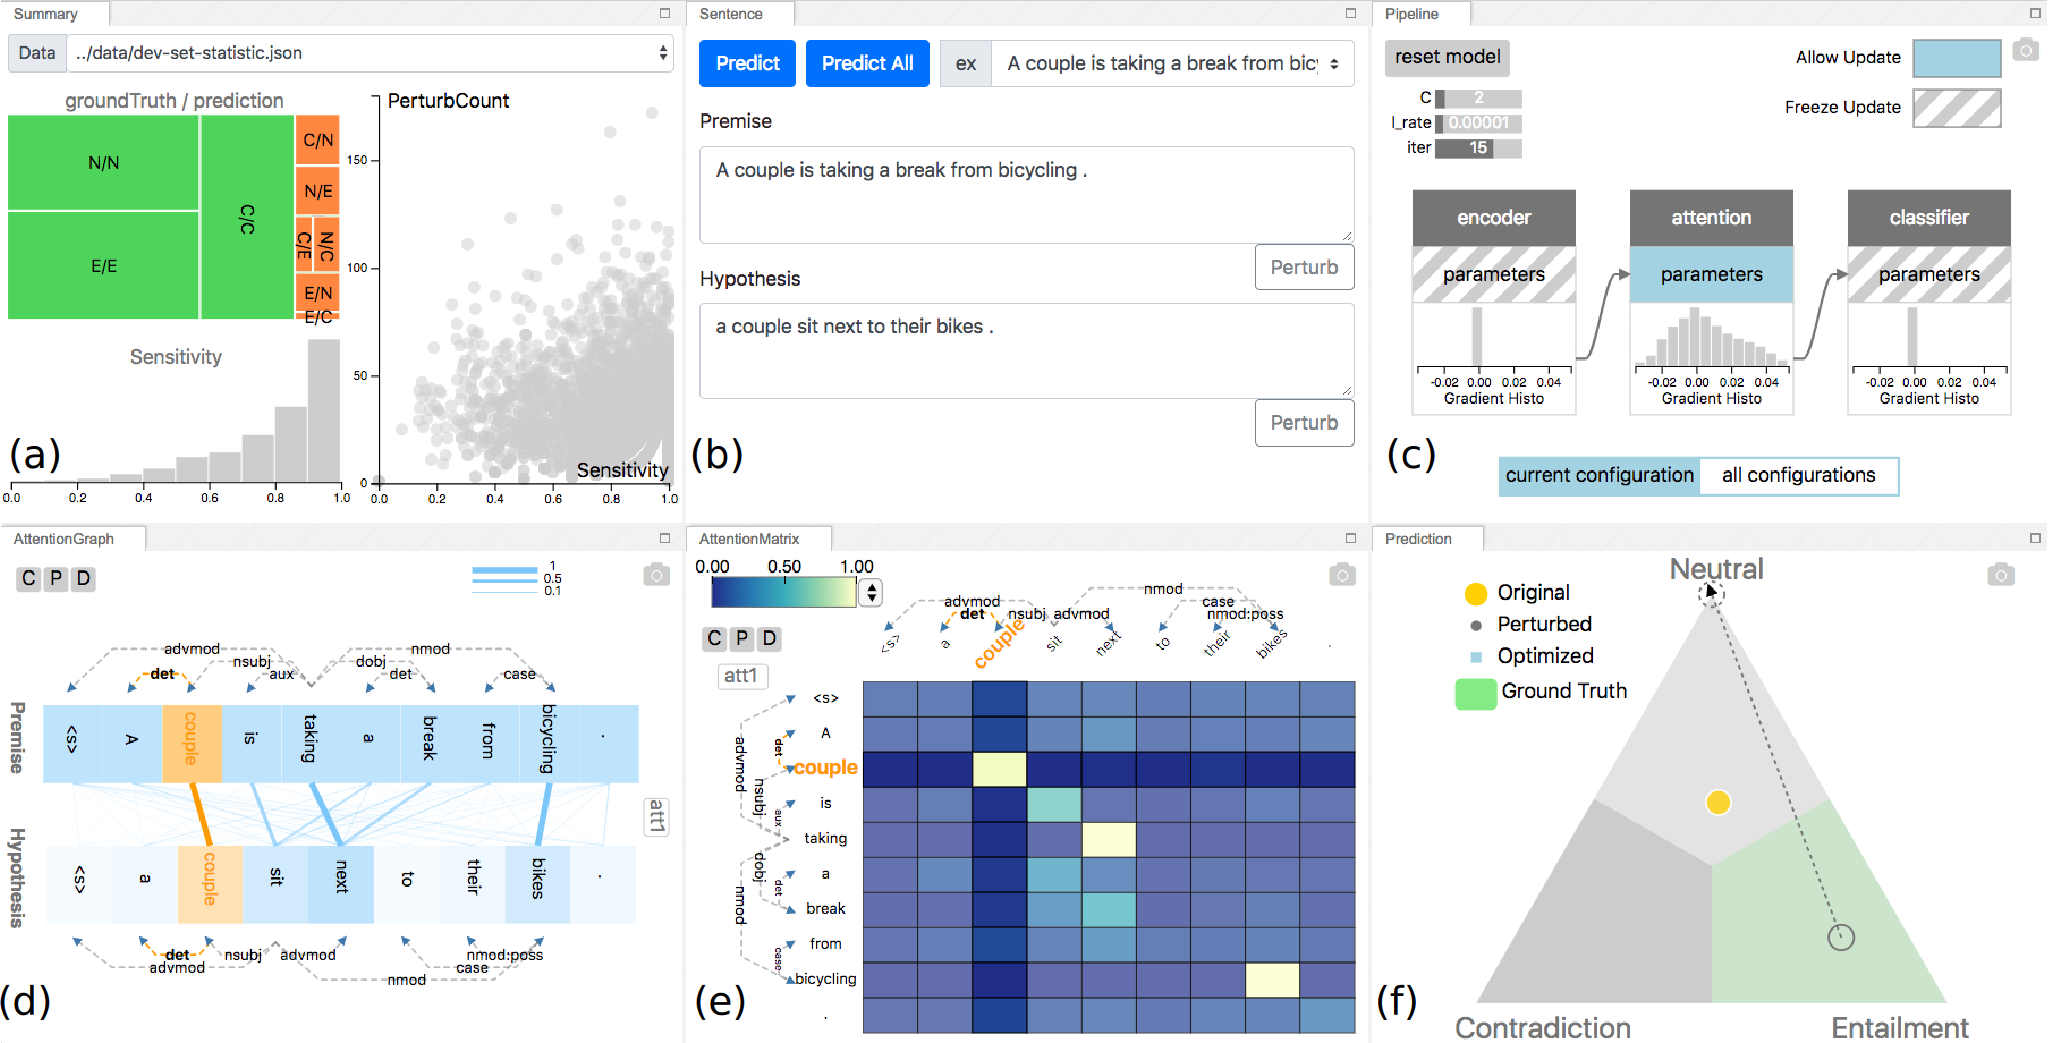
\includegraphics[width=0.78\linewidth]{teaser}
 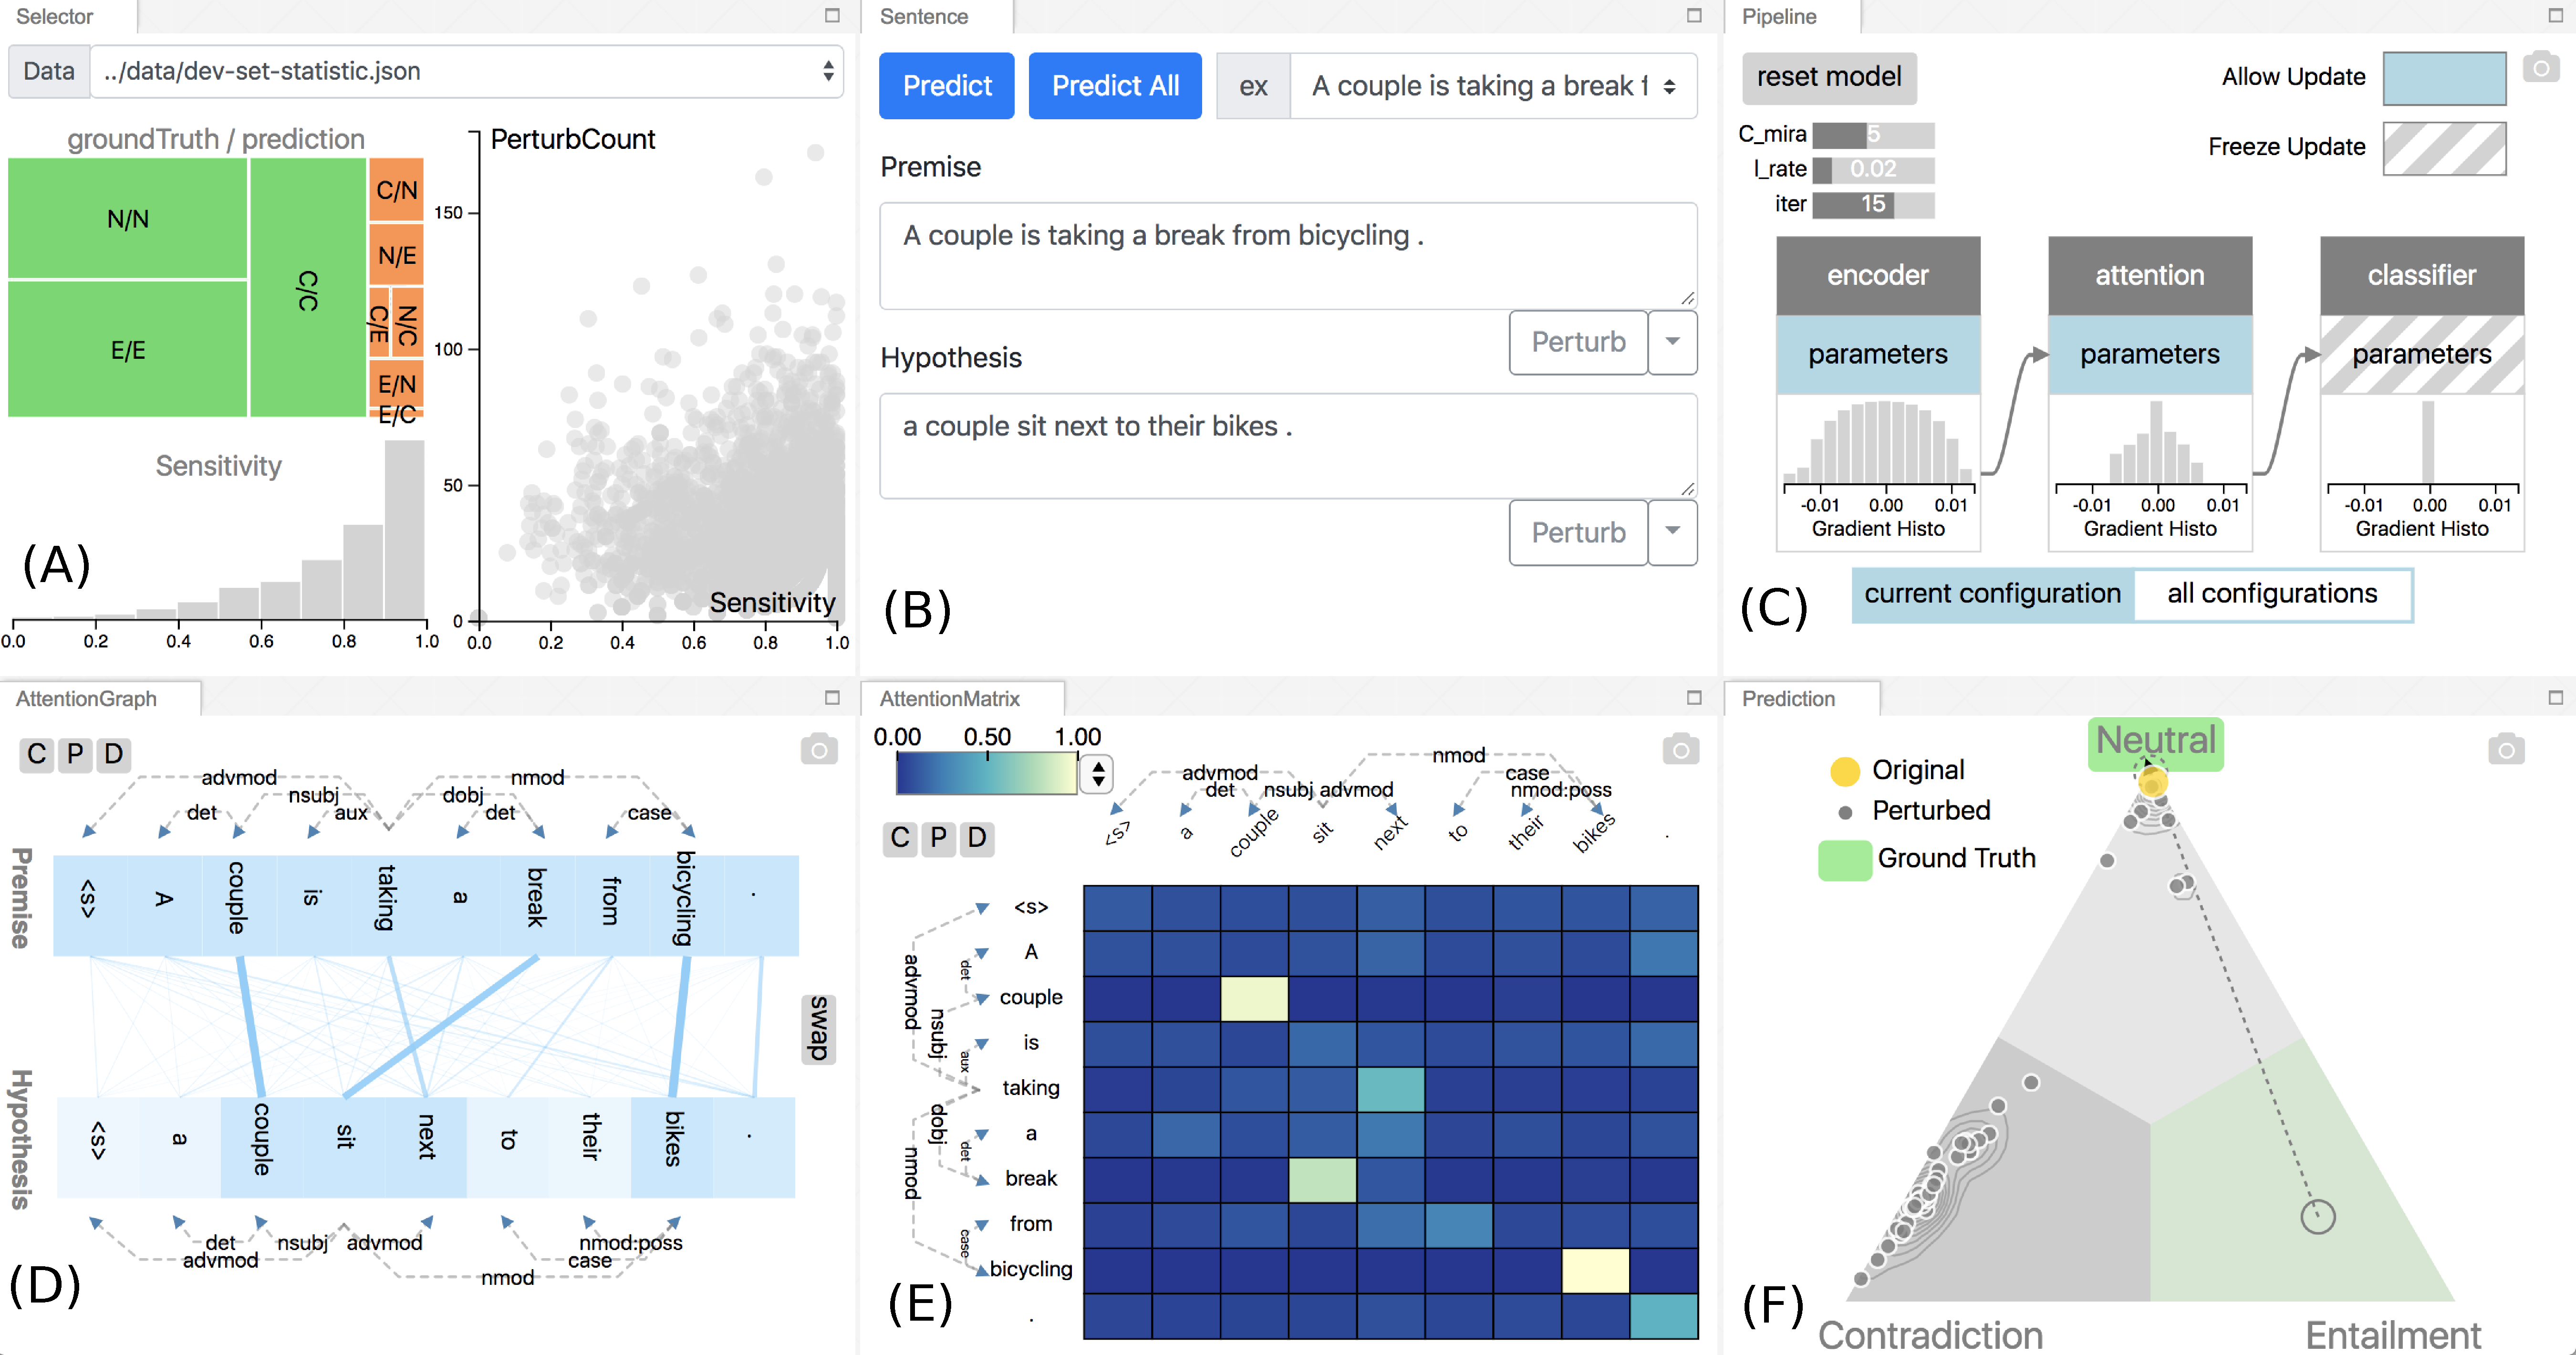
\includegraphics[width=1.0\linewidth]{teaser.pdf}
 \centering
 \vspace{-4mm}
  \caption{
The interface of the NLIZE system. During exploration, we can filter through a large number of sentence examples summarized in (A) and select examples of interest displayed in (B). The model internal information (attention) is displayed in (D) and (E). The predicted probability (one of three labels: \emph{neural}, \emph{entailment}, \emph{contradiction}) is shown in the barycentric coordinate in (F). Finally, the high-level model structure and the updates to the model are summarized in (C).
}
% \vspace{-2mm}
\label{fig:teaser}
}

%% Uncomment below to disable the manuscript note
%\renewcommand{\manuscriptnotetxt}{}

%% Copyright space is enabled by default as required by guidelines.
%% It is disabled by the 'review' option or via the following command:
% \nocopyrightspace

\vgtcinsertpkg

%%%%%%%%%%%%%%%%%%%%%%%%%%%%%%%%%%%%%%%%%%%%%%%%%%%%%%%%%%%%%%%%
%%%%%%%%%%%%%%%%%%%%%% START OF THE PAPER %%%%%%%%%%%%%%%%%%%%%%
%%%%%%%%%%%%%%%%%%%%%%%%%%%%%%%%%%%%%%%%%%%%%%%%%%%%%%%%%%%%%%%%%

\begin{document}

%% The ``\maketitle'' command must be the first command after the
%% ``\begin{document}'' command. It prepares and prints the title block.

%% the only exception to this rule is the \firstsection command
\section{Introduction}


exploration task

Comparsion with AllenNLP

\section{Background}
\label{sec:languageInference}

In order to full appreciate the technqiue discussed in this paper, certain background
in neural network and more specifically neural natural language process models are necessary.
In the following paragraphs, we aim to cover the most relevent backgound knowledge.

\shusen{high level NLP comments}

The grand challenge in Natural Language Processing (NLP) is to have machine to acquire
deep comprehension of textual information. Major tasks include Natural Language Inference,
Machine Translation, Questions Answering, Summarization, and etc.
Recently, neural networks models have performed strongly on these tasks.

Therefore, making sense and explaining predictions made by deep neural networks is not only
essential for validating and improving the model, but also becoming a necessity with
increasing demands for model accountability (e.g., what is the evidence for making the decision)
and model fairness (e.g., is the prediction affected by the bias in the training data).

% Recently, with the wide adoption of long-short term memory
% (LSTM) network and the introduction of attention mechanism,
% neural network based model have dominated nearly all linguistic tasks
% and thoroughtly refreshed many baseline performances.
% %
% However, the disruptive advance also brings enormous challenges.
% Netural network work based on has long been critizied for their opaque nature,
% and often been regarded as back box approach.
% Due to the opaque nature of the neural network model, interpret and making sense
% of many internal model mechanisms can be extremely challenging.

% \subsection{Neural Network Primer}

\begin{figure}[htbp]
\centering
\vspace{-2mm}
 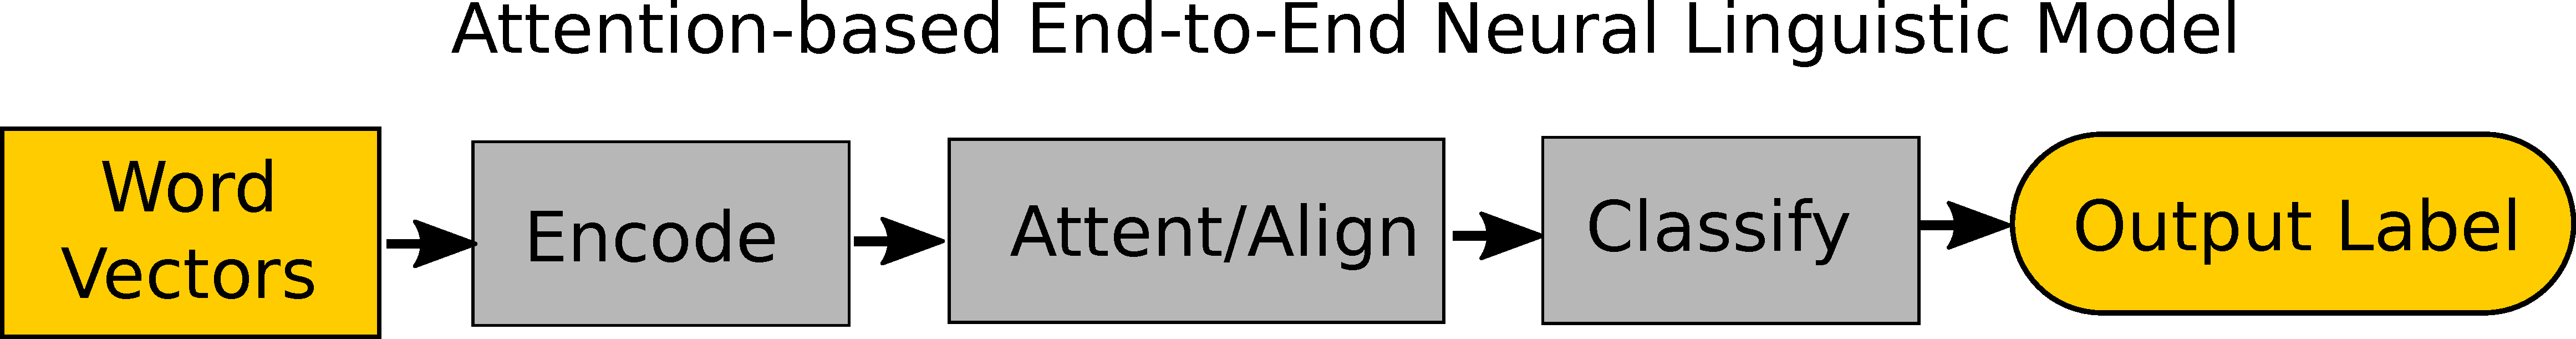
\includegraphics[width=1.0\linewidth]{end2end}
 \caption{End-to-end attention based model.}
\label{fig:modelPipeline}
\end{figure}

\subsection{Neural Network Model in NLP}
\shusen{neural linguistic models?}

\shusen{What is the basic understanding of neural network What is the end-to-end}

% \subsection{Interprebilty Challenges}
Compared with Conputer Vision, the discrete nature of words and sentences
presents additional challenge for
interpreting the model, since many visualization technique often employed
for images rely on continuous nature of the input space (e.g., one can interpolate
real values much easier than interplolate between words/sentences).
%
On the other hand, a majority of recent NLP neural networks share the nature of
end-to-end model, where the entire model operates as a black-box that takes
vectorized input and yields final prediction for a specific task.
Therefore, to study the inside of end-to-end neural models, it is important to
explore the interaction between intermediate representations and predictions.

The introduction of attention mechanism~\cite{bahdanau2014neural} allows
pairwise interaction between hidden states. This interaction can be naturally explained
as a form of alignment which exposes an interpretable layer in end-to-end neural networks.
Recently attention has contributed to many strongly-performed NLP models
~\cite{parikh2016emnlp},~\cite{rush2015neural},~\cite{yang2016hierarchical},
~\cite{seo2016bidirectional},~\cite{schwartz2017high}.
We will focus on its application in Natural Language Inference task as proposed in~\cite{parikh2016emnlp}.
However notice that our visualization can be generalized to other attention models as well.

\subsection{Natural Language Inference}
Natural Language Inference(cite?) is an important machine understanding task in NLP.
The problem definition is to classify the relationship between a premise sentence and a hypothesis sentence.
The prediction must fall in one of three catergories: $\{Entailment, Contradiction, Neutral\}$.
$Entailment$ refers to that the textual information of hypothesis is embedded in premise;
$Contradiction$ means the textuals of hypothesis opposes that of premise;
and $Neutral$ implies no conclusion can be made on either $Entailment$ or $Contradiction$.

Recently ~\cite{BowmanAngeliPotts2015} proposed a large dataset for this task. We will examine
the decomposable attention model~\cite{parikh2016emnlp} on this dataset with perturbation.

% showing an example??

\shusen{What is the most standard example to illustrate NLI problem?}

% \begin{itemize}
%     \item what is the textaul entailment problem
%     \item the importance of textual entailment problem
%     \item how easily can the visualization method extends other NLP problem
% \end{itemize}


\section{Related Works}
With the increasing demands for model accountability (e.g., what is the evidence for making the decision) and model fairness (e.g., is the prediction affected by the bias in the training data),
the interpretability of the machine learning model held significant implications. As a result, a wealth of researches have be focused on the explanation and interpretation of deep neural network models from both machine learning as well as visualization community.

\noindent\textbf{Model Interpretability.}
Before one can solve the model interpertability challenge, we first need to understand what constitute an explaination or interpretation of a machine learning model.
As discussed in ~\cite{Lipton2016, Doshi-Velez2017}, the concept of interprebale is inherently subjective, since the recipients of the explaination are always human.
% And the discussion of interpretability quickly become philosophical.
However, despite the underspecification nature of the problem, we can still refine the concept and provide certain guideline~\cite{Doshi-Velez2017}.

One of the most studied aread in model interpretability is the explanation of a given prediction.
Many works have been dedicated to providing intuitive explanations for a given prediction, several~\cite{RibeiroSinghGuestrin2016, KrausePererNg2016} of which approach the problem from a model agnostic approach that made them applicable to different applications (i.e., by fitting a simplier linear model near the prediction of interests).
%
Despite being invaluable for the providing human understandable explanation, the lack of the ability to access and explore the internal states of the model, which is vitally important to make sense of why a model fail, limits their ability for more in depth exploration and evaluation of the model.
% (Limitation of the state-of-the arts)
% Model independent explanations is useful to gain intuition, but they lack the ability to link the external observation with inner states/mechanism of the model.

\noindent\textbf{Visual Interpration of Neural Networks.}
The effectiveness in the exploration of complex relationships, visualization have long been adopted for interpreting neural network models (e.g., the early works such as~\cite{TzengMa2005})
Recently, many visualization works has dedicated to the neural network model interpretability challenges.
% The classification~\cite{KrausePererNg2016}
In the work~\cite{BilalJourablooYe2018} by Bilal et al., the authors analyzing classification errors in convolutional neural networks and answer the question on whether class hierarchy is learn in the network.
Liu et al.~\cite{LiuShiCao2018} explore the possiblility of understanding the training process of deep generative models.
The ActiVis~\cite{KahngAndrewsKalro2018} focus on large scale network in real world setting.
The DeepEyes~\cite{Pezzotti2018} focuses on the analyzing the training procss, so they can provide design guideline to the deep neutral network architect.

% \begin{itemize}
%     \item ActiVis: Visual Exploration of Industry-Scale Deep Neural Network Models
%     \item Analyzing the Training Processes of Deep Generative Models
%     \item Visual Diagnosis of Tree Boosting Methods
%     \item TreePOD: Sensitivity-Aware Selection of Pareto-Optimal Decision Trees
%     \item LSTMVis: A Tool for Visual Analysis of Hidden State Dynamics in Recurrent Neural Networks
%     \item Do Convolutional Neural Networks learn Class Hierarchy?
%     \item DeepEyes: Progressive Visual Analytics for Designing Deep Neural Networks
% \end{itemize}

\noindent\textbf{Neural Linguistic Model Visualization.}
Compare to the multitude of researchs for making sense of convolutional neural networks, relatively less works has been dedicated to neural linguistic models.
%
However, the previous works~\cite{KarpathyJohnson2015, LiChenHovy2015, StrobeltGehrmannPfister2018, LiuBremerJayaraman2018} not only demonstrated the benefit of visualization in understanding NLP models, but also revealed enoumous possibility for future applications.
% There is many unresolve challenge and the
The early work on charactor level recurrent network~\cite{KarpathyJohnson2015} demonstrates effectness of the hidden state in capturing the unique pattern in training text. The compositionality exibited in neural linguistic model (i.e., build sentence from meaing of words and phrases) are examined in the work by Li et al. ~\cite{LiChenHovy2015}, by utilizing methods inspired by similar work in computer vision.
The LSTMvis~\cite{StrobeltGehrmannPfister2018} work utilized a line plot style visual encoding to visualize the time varying hidden states of recurent neutural network. The word embedding visualization work~\cite{LiuBremerJayaraman2018} illustrate how semantic relationship can be recovered by linear projections in the high-dimensional word embedding space produced by word2vec~\cite{MikolovSutskeverChen2013} or glove~\cite{PenningtonSocherManning2014}.


\section{Task Analysis}
\label{sec:task}
Identify the analysis goals and the corresponding visualization tasks is the first yet significant step in designing a useful tool. In this section, we examine how domain experts normally approach the task of analyzing a model (i.e., assess its strength and weakness) and identify where and how an interactive visualization system can aid in such a process.
Then, we reify the multitude discussion with domain experts into concrete tasks, which guide the design and implementation of the proposed tool.

During our long-term collaboration with NLP experts, we have conducted extensive discussion to understand the common approach employed by researcher for assessing the behavior of a model.%
The prediction accuracy has its place as an objective evaluation metric to measure the overall effectiveness of the model, however, the accuracy number alone does not provide the full story.
For example, the model may produce correct predictions for the ``wrong'' reasons (e.g., pickup unintended pattern in the training data that can not be generalized in real word scenarios).
%
As a result, the domain experts often rely on exploration centric approach to
conduct error analysis and obtain intuition.

There is little one can learn when everything is behaving as expect, therefore,
observing how model make mistakes under various scenarios is at the center of such a process.
The experts often start with simple failure examples, and then make minor perturbations (replace a word or phrase) to the input and observe the change in the prediction. This exercise help isolate where in the input is likely contributed to the failures. For many NLP models, the attention information (see Section~\ref{sec:attention}) is essential to infer the mechanism of the model. The expert can print out the attention values or generate plots to visualize the alignment between sentences or compare attentions. As the experts explore more variation of similar examples, combined with their domain knowledge, he / she may develop hypotheses about the cause of failures, or ask additional questions, which lead to further experimentation.
%
The requirement for such exploratory analysis meshed nicely with the benefit of interactive visual exploration, in which the user can make adjustment on-the-fly and obtain instantaneous visual feedbacks that encode various model information.
%
Moreover, by introducing new visual encoding and summarization, we can drastically expand the ways domain experts interact with the model, enable exploration options that is not possible before either due to tedious manual operation or lack of communication channels.

%Through many rounds of discussions with NLP experts,
In such a highly exploratory process, the expert likely will have many ``what if'' type of questions (e.g., what if I make change to this word in the input, what if I force the words to align correctly in the attention), get responsive answers to these queries is essential to maintain the flow of reasoning.
%
Here, we solidify the analysis goals around the support for these type workflow and thought process of the experts.
%
\begin{itemize}
\item Firstly, understanding how perturbation (e.g., replacing words) of the input affect the prediction is the curial part of error analysis. It not only measures the prediction sensitivity, but also help reveal the potential source of the errors in the input (\textbf{T1}).

%Understand how attention affect the prediction.
\item Secondly, study the role and mechanism of attention by examine how variation in the input affect the attention, and how changes in attention affect prediction (\textbf{T2}).
%Study the relationship between model stages (encoder, attention, classifier) and the prediction
So far, we focus on how changes in earlier stage of the model affect later stages or final prediction.

\item However, what if the current prediction is wrong, how can we apply minimal update to the model to produce correct prediction and how would such a modification affect attention.
Therefore, thirdly, we want to explore how model should be updated to produce the desirable change of prediction, and how the attention respond to such a change (\textbf{T3}).
\end{itemize}
%
% Based on the NLP analysis goals, we identify the visualization tasks to achieve these goals.

% \begin{itemize}
% \item \textbf{T1} Visualize the \emph{input}, \emph{attention}, \emph{prediction} of the model.
% \item \textbf{T2} Automate the perturbation of the input, explore the perturbation result.
% \item \textbf{T3} Customize the \emph{attention} for studying the relationship between attention and prediction
% \item \textbf{T4} Visualize the changes in the model stages with respect to prediction change driven model update %\shusen{does not make sense}
% \end{itemize}


%interrupted when they can not easily receive the answers to their immediate queries.

% examining examples (e.g, what are the mistakes made by the model), and conduct experiments (e.g., perturb the input and observe the changes), formulate hypothesis (e.g, what are the potential causes for the failure).
%ultimate forms intuition about the strength or the weakness of a given model.
% , then additional examples or variation of existing examples are bring in to rejected or confirm the hypotheses. And new questions or hypothesis may arise.
%Such an analysis is iterative in nature and guided by domain knowledge and hypotheses based on the architecture. As they ask more questions and experiment
%experiment with model iterate their understanding of the model behavior, ultimate forms intuition about the strength or the weakness of a given model.
%and come up hypothesis about the potential cause for the failure.



%\begin{figure}[htbp]
%\centering
%\vspace{-2mm}
% 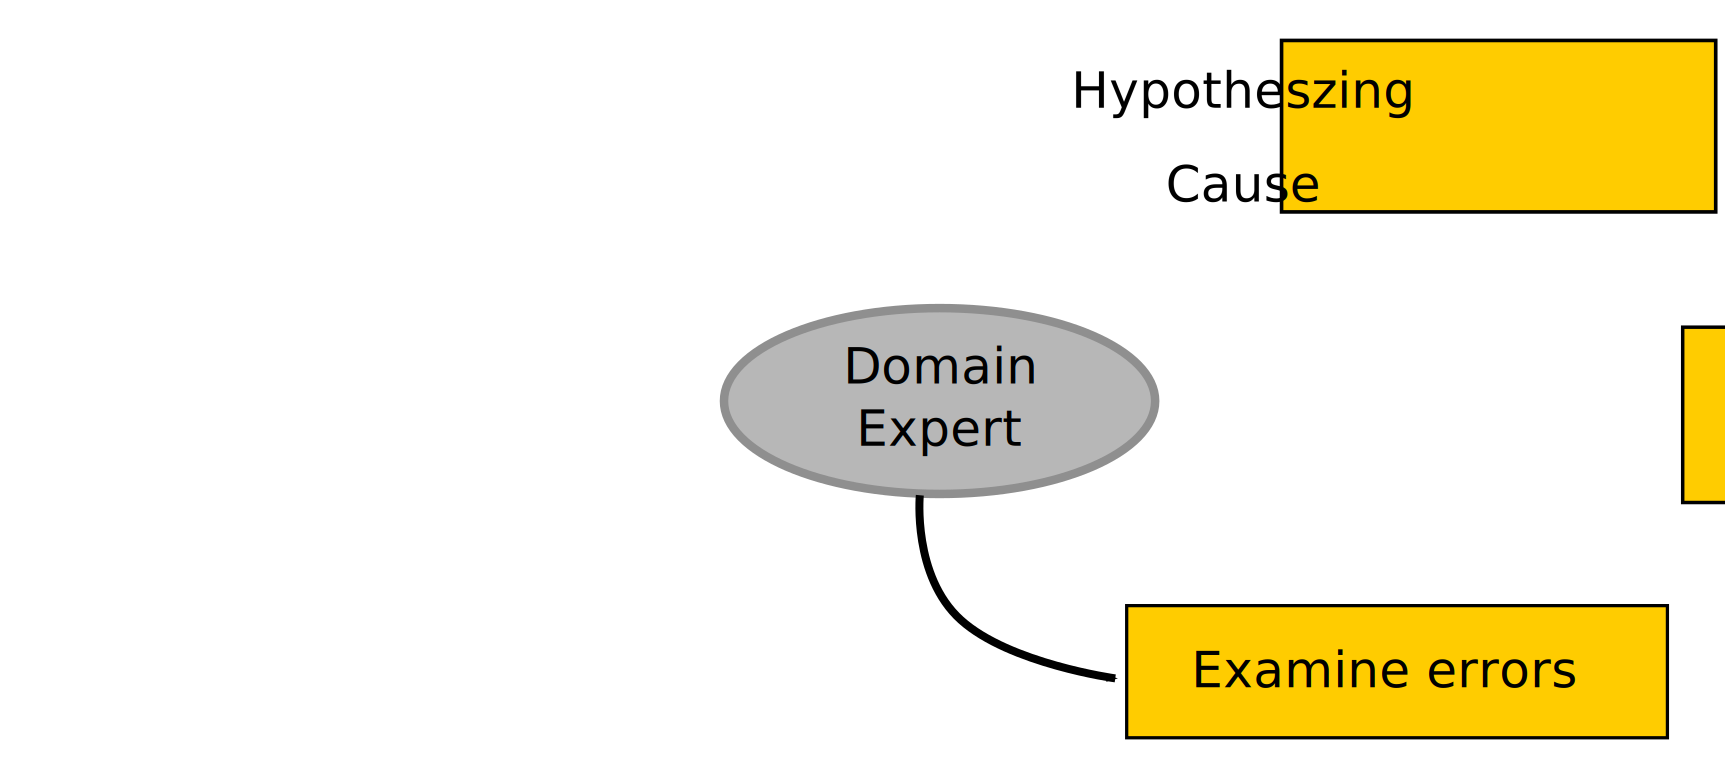
\includegraphics[width=1.0\linewidth]{errorAnalysis}
% \caption{How domain experts conduct error analysis on the model.}
%\label{fig:modelPipeline}
%\end{figure}

\section{NLIZE System}
In this section, we discuss the design and implementation of the NLIZE (pronounced as ``analyze'', see interface overview in Fig.~\ref{fig:teaser}) system, which address the visualization tasks (\textbf{T1-3}).
%
As discussed in the task analysis, the experts often analyze and obtain intuition about the model by studying how altering one part of the model affect other stages of the pipeline.
%
Such a process can be generalized as the perturbation-driven paradigm, which is used as guiding principal for designing the proposed tool.
%
As illustrated in Fig.~\ref{fig:modelPipeline}, we enables the automated or user-guided \emph{perturbation} (i.e., replace words) of the input sentence, the \emph{perturbation} of attention (i.e., alter the alignment between sentences)inside the model, as well as the \emph{perturbation} the prediction (e.g., adjust the prediction by making updates to the model).
%
In the following sections, we describe in detail the five major components of the proposed system, namely, sentence view  (Section~\ref{sec:sentence}), attention view (Section~\ref{sec:attention}), prediction view (Section~\ref{sec:prediction}), pipeline view (Section~\ref{sec:pipeline}), all pair summary view (Section~\ref{sec:allPairs}).


\begin{figure}[htbp]
\centering
 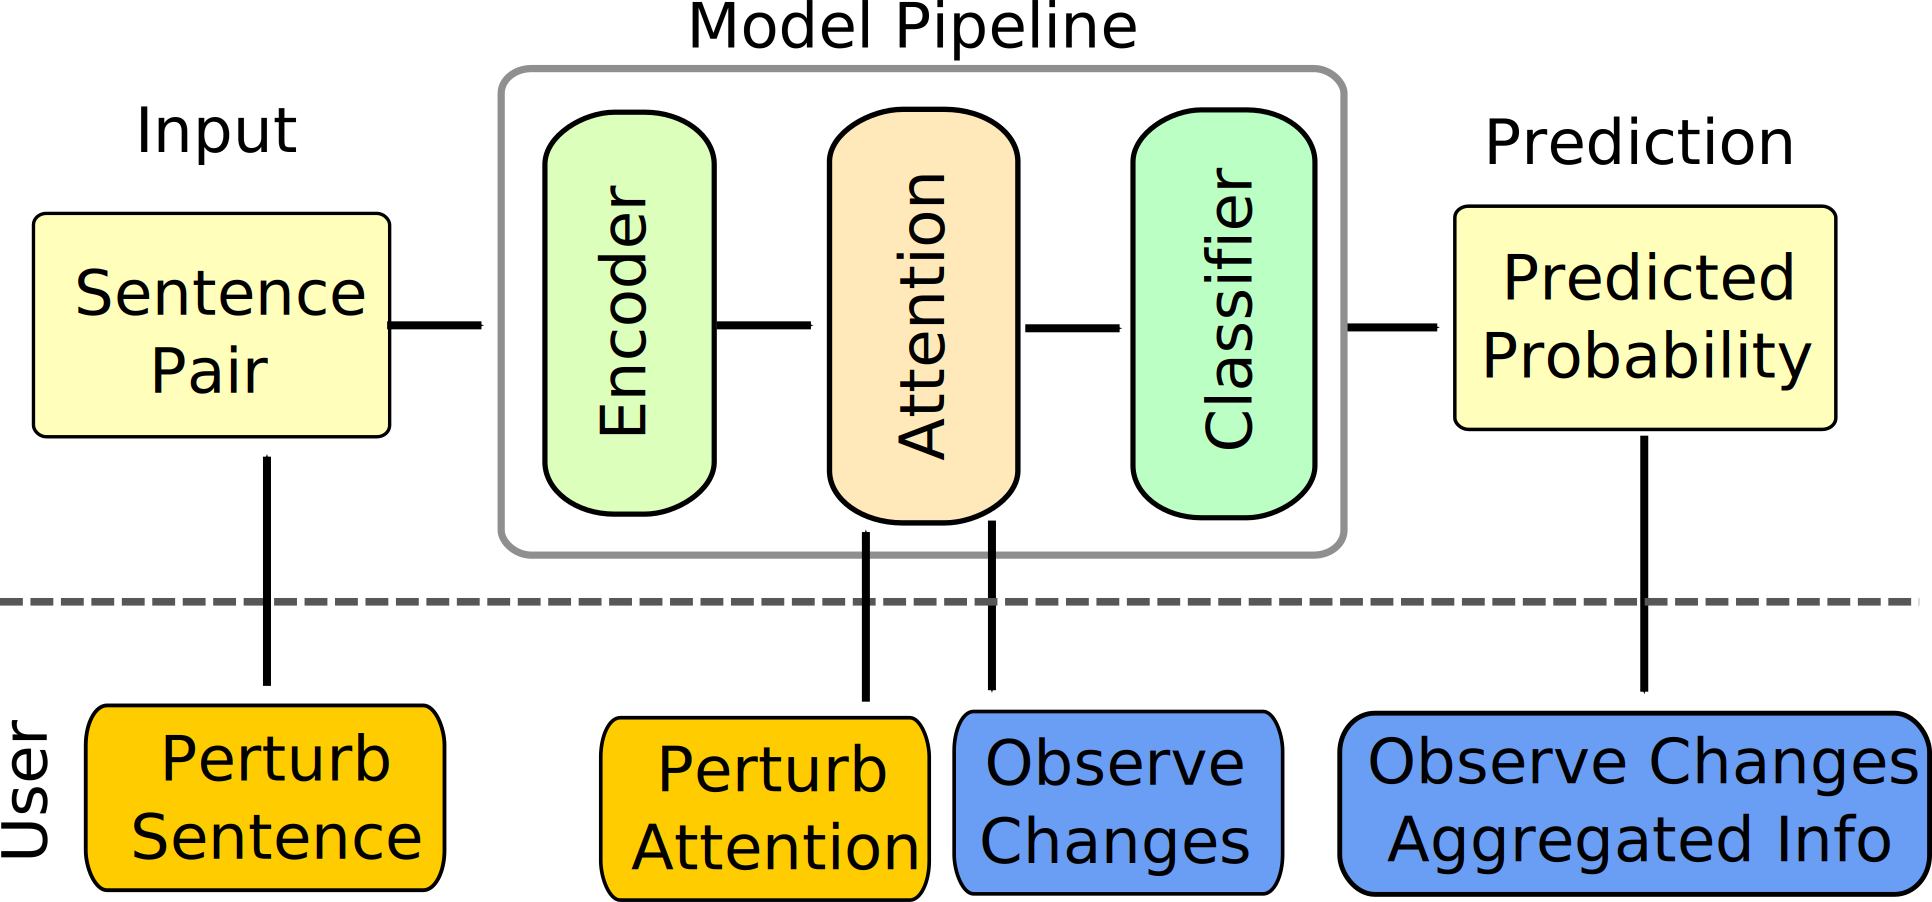
\includegraphics[width=1.0\linewidth]{pipeline}
 \caption{
 Perturbation-driven exploration of the natural language inference model.
 In the proposed tool, we enables the interrogation of the relationship between different components of the model via the perturbation-based analysis.
 %
 The user can perturb the of the input sentence (i.e., replace words with synonymous), perturb the attention (i.e., alter the soft alignment between sentences), and perturb the prediction (i.e., adjust the prediction by making updates to the model).
}
\label{fig:modelPipeline}
\end{figure}

% Beside looking into the internal states, understanding how each of the component of the model interact with input and output as well as with each other is the crucial for truly examine the mechanism of the model.
%
% Look at how the model work in action and interrogate relationship between different component, i.e., how the change made to one part of model affect the other pieces present, is the key to gain the full picture.


\subsection{All Pairs Summary View}
\label{sec:allPairs}
Since we can only focus on one individual example at a time for detail analysis, 
how to pick an single pair of sentence from the development or test dataset (for the SNLI dataset, each of the these set consists of close to $10k$ examples) is an obvious challenge.
%
In addition, we also want to obtain certain high-level understand of how the whole set behave, beyond the information the prediction accuracy provide.

%The all pair
\begin{itemize}
\item How to go from 10k pair to one pair
\item What constitute interesting example
\item How to get a sense of overall prediction result
\end{itemize}

\subsection{Sentence View}
The sentence view shows the premise and hypothesis sentences, and in case of the existence of perturbation, highlight the where in the sentence the perturbation happens.
%
Add user customized sentences.

\begin{itemize}
\item Examine perturbed pair
\item See which word is perturbed in a sentence
\item Add to existing example collection
\end{itemize}



\subsection{Attention View}
\label{sec:attentionView}
As discussed in Section~\ref{sec:attention}, the attention is the only intermediate layer in the network that provides interpretable information for domain experts to infer the inner mechanisms of the model.
%
Intuitively, the attention captures the alignment of words between input sentences. For the NLI model examined in this work, the attention is represented as a matrix, in which the entries in the $i^{th}$ row correspond to the probabilities of words in the hypotheses aligned to the $i^{th}$ word in the premise.

As illustrated in Fig.~\ref{fig:attentionVis}, we employ graph and matrix two visual encodings for visualizing attention. In the graph attention view (Fig.~\ref{fig:attentionVis}(a)), a bipartite graph encoding is adopted, in which the edge thickness corresponds to the attention value. The color of the rectangle text block encodes the sum of all edge values connected to it (darker shade of blue corresponds to higher values).
%
The graph view is good for highlighting the most dominant alignments. However, if many attention values are high, the edges may become cluttered, leading to less effective visualization. Also, if the sentence structures between premise and hypothesis are drastically different, we are likely to see the prominent edges cross each other, which can also lead to confusing and misleading visual patterns.
%
The matrix attention view (Fig.~\ref{fig:attentionVis}(b)), despite being more verbose and less efficient in highlighting the dominant alignment, does not have similar shortcomings. However, extra effort may be required for identifying the words that correspond to high-value entries in the matrix. Together, the graph and matrix views complement each other and provide the same information from different perspectives (a related matrix/graph visualization scheme is presented in \cite{MaKenyonForbes2015} for studying the brain network). 
%As illustrated by the pink arrowed lines, we can see how the same attention value is visualized in both the graph and the matrix view.
To help the user recognize the correspondence during the exploration, we enable the linkage between highlighted actions in both views (see Fig.~\ref{fig:attentionVis}(a)(b), the attention of the two ``couple'' is highlighted).

To support the ability to perturb the attention values (\textbf{T2}), we include the attention editing functionality. The attention matrix view is the most suitable place to conduct the editing operation since it provides a direct mapping of the attention value.
As we can see in Fig.~\ref{fig:attentionVis}(c), when a user clicks the cell of the matrix, a sider will pop up for customizing the attention value (as the user edits the value, each row is automatically renormalized).
%
As illustrated in Fig.~\ref{fig:attentionVis}($a_{2}$)(f), we also allow the user to compare currently and previously displayed attentions by computing and visualizing their cell-wise differences (the user can toggle between different display modes using the C (current), P (previous), D (difference) buttons bellow the colormap).


Even though the attention does not explicitly encode any grammar, it often highlights essential words in the sentence structure.
%
To help the researcher better understand the relationship between attention and sentence structure, as illustrated in Fig.~\ref{fig:attentionVis}($a_{1}$), we overlay the grammar dependency tree~\cite{Nivre2005} structure next to the sentence.
%
Since the dependency tree encodes the word importance information in a hierarchical manner, it is very suitable for sentence simplification tasks.
Here, we utilize the grammar dependency tree to trim the decorative structure to shorten the sentence to combat the visual clutter when examining long sentences (see Fig.~\ref{fig:attentionVis}(d)). A simplification example is shown in  Fig.~\ref{fig:attentionVis}(d)(e)(f).


%\subsubsection{Attention visualization challenges}
% \begin{itemize}
% 	\item Why we need two different visual encoding to visualize attention? bipartite visualization more easier to highlight the
% 	\item long sentence, collapse
% 	\item quickly compare the alignment information with the sentence's linguistic structure.
% \end{itemize}


% \subsection{Interpret Attention Via Model Perturbation}
 % how to encode the information
\subsection{Prediction View}

\begin{figure}[htbp]
\centering
\vspace{-2mm}
 
\includegraphics[width=0.85\linewidth]{predictionView}
 \caption{How domain experts conduct error analysis on the model.}
\label{fig:modelPipeline}
\end{figure}


\subsection{Pipeline View}

\begin{figure}[htbp]
\centering
\vspace{-2mm}
 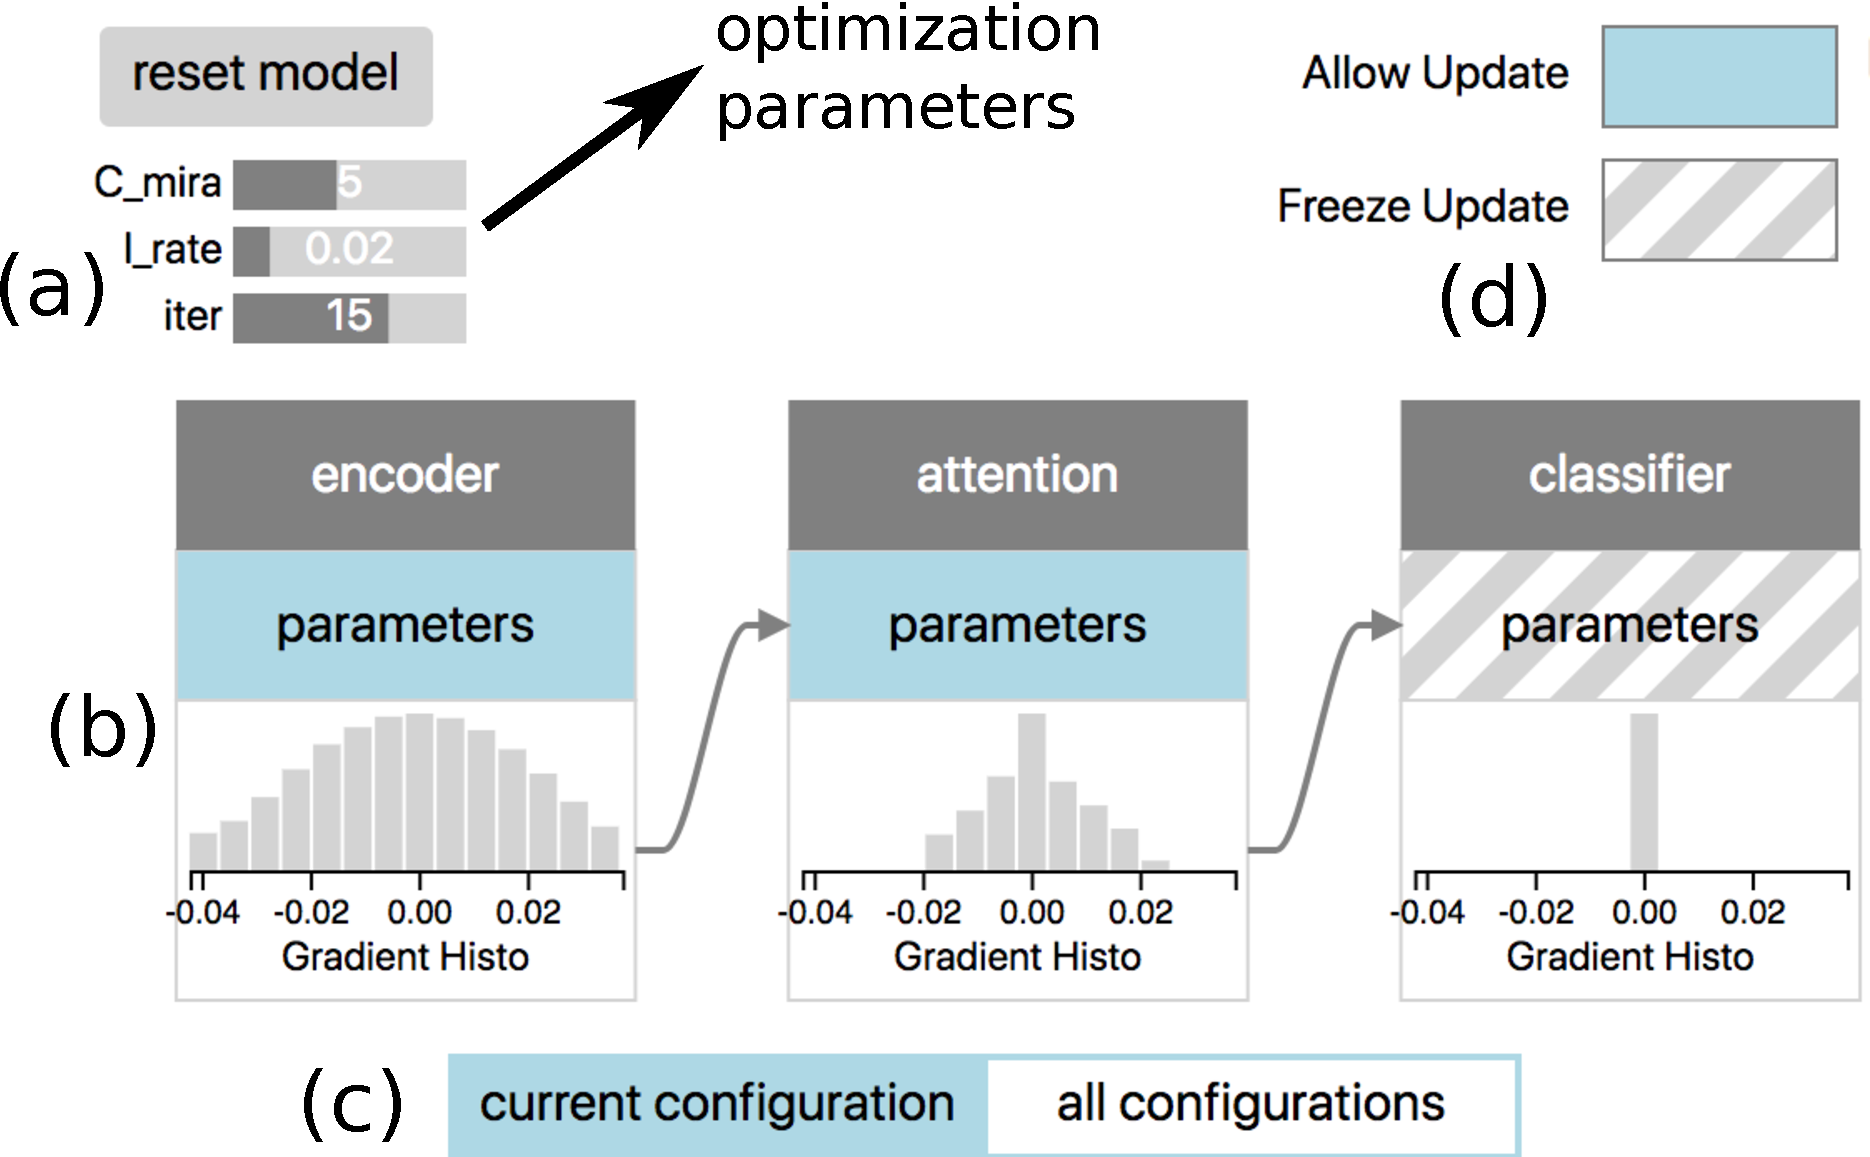
\includegraphics[width=1.0\linewidth]{pipelineView}
 \caption{Visual representation of the three stage pipeline.}
\label{fig:modelPipeline}
\end{figure}

\subsubsection{Margin-Infused Relaxed Algorithm (MIRA)}
the mira loss is $|w' - w|^2 + C * J(w')$

\section{Pipeline}

\subsection{All Predictions Summary View}
\label{sec:allPairs}
Since we can only focus on one individual example at a time for detail analysis,
how to pick an single pair of sentence from the development or test dataset (for the SNLI dataset, each of the these set consists of close to $10k$ examples) is an obvious challenge.
%
In addition, we also want to obtain certain high-level understand of how the whole set behave, beyond the information the prediction accuracy provide.

\begin{figure}[htbp]
\centering
\vspace{-2mm}
 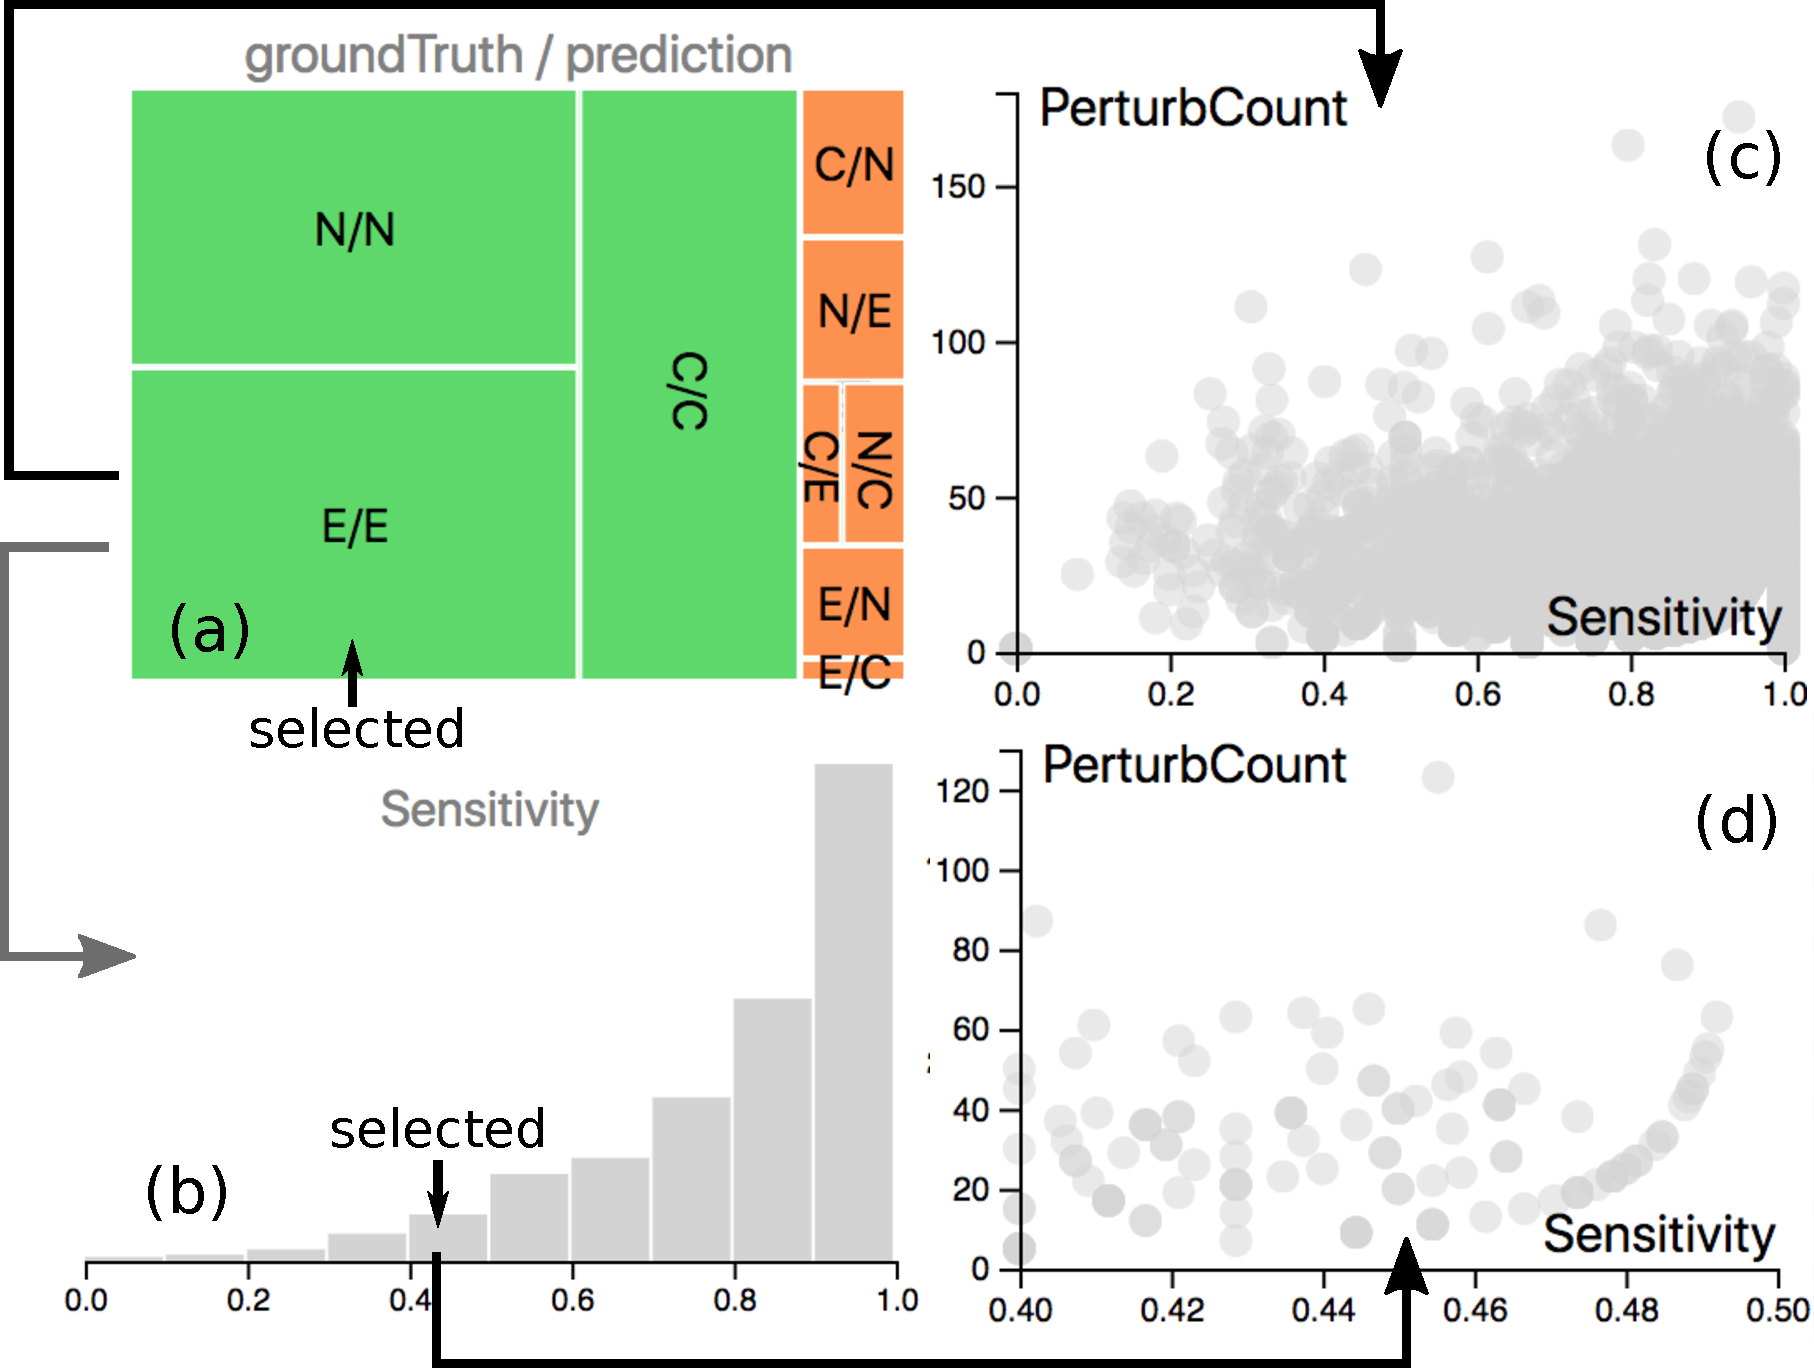
\includegraphics[width=1.0\linewidth]{summaryView}
 \caption{Explore the full development set and examine their prediction result and sensitivity.}
\label{fig:modelPipeline}
\end{figure}

%The all pair
\begin{itemize}
\item How to go from 10k pair to one pair
\item What constitute interesting example
\item How to get a sense of overall prediction result
\end{itemize}

\subsection{Implementation}
\label{sec:implementation}


\section{Application Scenarios}
\label{sec:caseStudy}
% \shusen{A full case study that driven by the visualization task and the question associated with them}
%In this section, we discuss application scenarios, in which the domain experts utilize the 
To better illustrate how the proposed perturbation-driven exploration tool helps the domain experts interpret the neural network model, we present five application scenarios gathered by the domain experts who integrated the proposed tool into their model analysis workflow.

\begin{figure}[htbp]
\centering
\vspace{-2mm}
 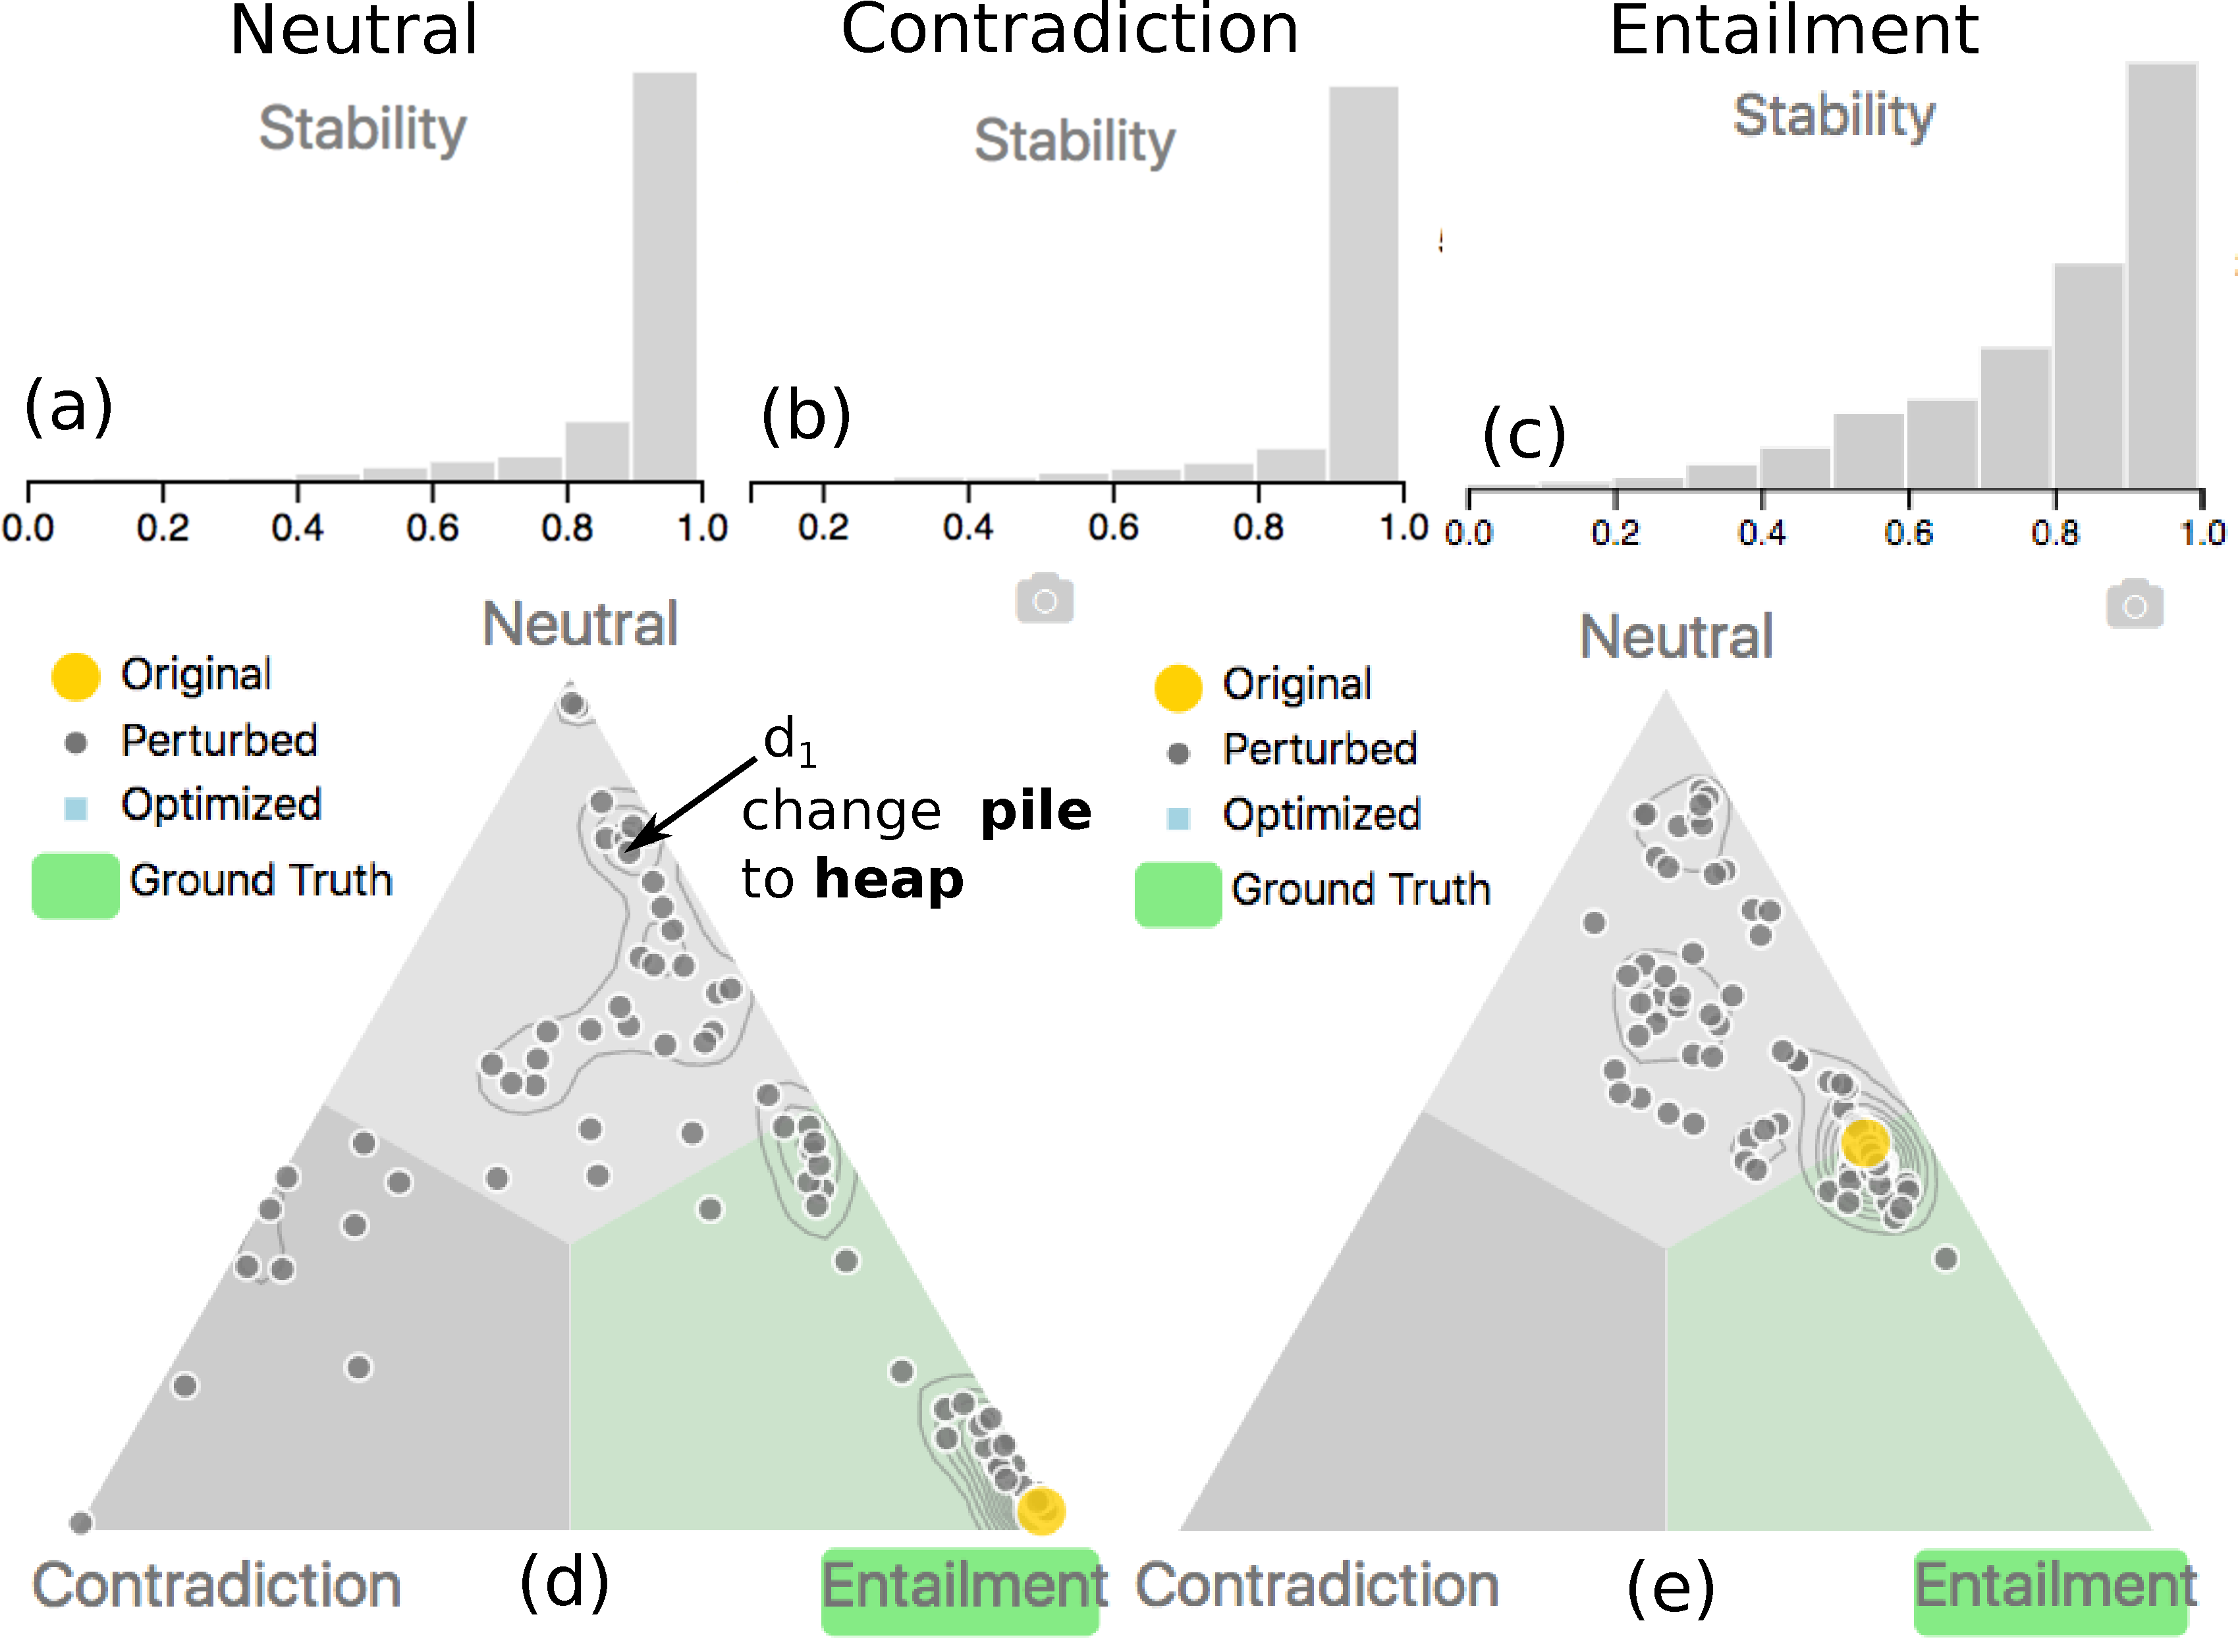
\includegraphics[width=1.0\linewidth]{predictStability}
 \caption{
Prediction stability assessment. Isolate unstable one
 }
\label{fig:pipelineView}
\end{figure}

\subsection{Scenario 1: Assess the Model Prediction Stability}
Utilize input sentence perturbation to assess the overall stability of the prediction

\subsection{Scenario 1: Interpreting Decision Making Process}
Understand how the model arrive at the prediction is the first step  only essential for evaluating the model performance but also necessary for hypothesizing improvement strategies.
%
The three stages (encoder, attention, classifier) of the model work in synergy to produce the correct prediction.
%
%One of the essential task for can be made in either of these stages.
% \shusen{difference in sensitivity among entail natural and contradict relationships}
% the generate the correct prediction for the wrong reason

\subsection{Scenario 2: What Does It Take to Correct a Wrong Prediction?}
In the previous section, we discussed how we can use forward prediction



\subsection{Scenario 4: Handcraft Example Analysis}
Well-known tough examples, such as the Facebook IPO example discussed in Section~\ref{sec:background}.

\subsection{Scenario 5: Explore Relationship Between Grammar and Attention}
Can attention capture grammar structure? Is 
%\subsection{Is the Prediction Stable?}
%\subsection{Where Are the Mistakes?}
%\subsection{How Attention Affect the Prediction?}
%\subsection{What Does It Take to Change the Prediction?}
%\subsection{Is Attention All You Need?}


\section{Evaluation and Feedback}
%The motivation for designing the proposed tool is the error analysis challenges faced by our long-term collaborators working on natural language inference research. During the entire design and development process, we worked closely with two NLP experts, and their constant evaluation and feedback have helped shape the tool we see today. 
%
As discussed previously, we have worked closely with NLP experts during the development of the tool. However, since these two NLP experts have been heavily involved in the design process, they may not be the best candidates for identifying potential issues of the tool due to familiarity.  To uncover the limitation and identify areas for improvement, we gathered a wider audience from either visualization (4 researchers, including 3 Ph.D.-level students and one postdoc researcher) or NLP backgrounds (5 Ph.D.-level students who are familiar with the concept of natural language inference and attention) for obtaining feedback for the tool.  

With the goal to identify the potential interface design issues, we first conducted an informal demonstration-and-feedback session with the visualization group. We started by explaining the basic natural language inference concept. We then demonstrated the features of the tool in detail. After that, we answered questions and seek feedback.
%
From this session, we have gathered complaints and suggestions on various aspects of the visual interface. Some of the identified issues include: (1) difficult to distinguish different types of predictions (distinct colors are added to the final version); (2) hard to recognize the ground truth label (we now use a green rectangle to indicate the ground truth); (3) lack of legends to understand the key elements in plots (legends are added). We address these interface issues before presenting the final version to the NLP group.

We conduct an individual revaluation session with each participant from the NLP group, in which the participant is given 30 minutes to experiment with the tool after an overall feature demonstration. 
%
Since both the matrix and graph-based visual encodings are the most common attention representations used in the NLP literature, most participants can utilize them immediately and find the linked highlighting feature of the two views quite useful.
% 
Once the participants familiarize with the tool, they often try to type two similar sentences and examine the attention and prediction. After that, they will modify some words, or negate the hypothesis sentence, and then check the attention and prediction again.
%
Such a ``perturb and observe'' operation demonstrates the most fundamental exploration strategy and matches well to the perturbation-driven paradigm the proposed tool aims to support.

One participant shows us two examples after a quick exploration session. 
In the first example, he identifies a case where the wrong attention alignment produces a correct final prediction.
%
In the other example, he finds a sentence pair with the incorrect attention that produces a wrong prediction. 
However, even after he forces the correct alignment, the prediction result remains incorrect. He believes observations such as these will provide valuable insights for him to interpret the model. 
%
Another participant comments that the ability to enable or disable model parameter update in the pipeline view is beneficial.

The participants also identify potential issues and places for improvement. 
One participant wishes the pipeline view could provide more detailed information compared to the current aggregated histogram visualization. 
Another participant suggests the possibility to examine multiple similar examples at a time (instead of one by one). 
%
Also, for the participants who do not focus on NLI research, understanding all the views at first can be a bit challenging. However, this issue can be addressed by the modular design, as the user can simply enable, only the sentence, attention, and prediction views.
%
Overall, all the participants believe the proposed tool is very convenient for conducting experiment and exploring various hypotheses, which is essential for building intuitions about the model.




\section{Discussion}

The current setup for the proposed tool is only suitable for natural language inference task. However, due to the modular design and the many shared attribution among end-two-end NLP models we can readily extends the system to handle other tasks. We plan add support for neural machine translation, question and answer, and more in the future.
%
Initial setup cost and learning curve of the tool are often the major barriers for visualization adoption.
In the proposed system, we approach these challenges by designing the system as an python library rather than as an monolithic tool. 
Just like a python plotting library, the different pieces of the visualization can be access individual or combined in any ways by the user via a simple python API.
As a result, the proposed tool can not only be configured to suit the different needs of the individual domain experts to better fit into their workflow, but also enable NLP researchers to experiment to simpler features reduce the learning curved. 
Finally, the researchers are really appreciated the ability to easily swap functionality of the visualization in python.
%defined and combined  The long term goal for the 

How to generate meaningful perturbation
Limitation: sometime wordNet produce not very meaningful  perturbations

%\begin{itemize}
%    \item how the visualization approaches generalizes to other NLP task
%    \item limitation
%    \item future direction
%\end{itemize}
 % how to encode the information



%% if specified like this the section will be committed in review mode
% \acknowledgments{
% The authors wish to thank A, B, and C. This work was supported in part by
% a grant from XYZ (\# 12345-67890).}

%\bibliographystyle{abbrv}
\bibliographystyle{abbrv-doi}
%\bibliographystyle{abbrv-doi-narrow}
%\bibliographystyle{abbrv-doi-hyperref}
%\bibliographystyle{abbrv-doi-hyperref-narrow}

\bibliography{entailVis.bib}
\end{document}
